\documentclass[12pt,a4paper]{article}
\usepackage{geometry}
\usepackage{ctex}
\usepackage{fontspec}

\usepackage{hyperref}
\usepackage{xcolor}
\usepackage{enumitem}
\usepackage{graphicx}
\usepackage{titlesec}

% Reduce section* title font size and spacing
\titleformat{\section}[block]{\bfseries}{\thesection}{0.5em}{}
\titlespacing*{\section}{0pt}{5pt}{0pt}

% Custom commands for formatting
\newcommand{\ResumeItem}[2]{\noindent\textbf{#1} \hfill {\small #2}\\}
\newcommand{\GrayText}[1]{\textcolor{gray}{#1}}

\geometry{left=2.5cm,right=2.5cm,top=2.5cm,bottom=2.5cm}
\setmainfont{Times New Roman}
\setCJKmainfont[Scale=1]{Kaiti SC} % 12pt * 1.17 ≈ 14pt for CJK

% Increase line spacing globally
\linespread{1.2} % Increase line spacing (default is 1.0)

% Reduce spacing in lists
\setlist{nosep,itemsep=0em,topsep=0.2em,parsep=0em,partopsep=0em}

% Remove page numbers
\pagestyle{empty}

\begin{document}
{
  \noindent
  尊敬的博士生导师:

  您好!我申请审核制攻读博士学位,申请主要研究方向:密码算法软硬件优化实现、密码算法侧信道攻击与防御、轻量级密码算法设计与分析等。以下是个人信息与科研情况,迫切想通过读博进一步提升自己,望老师给予机会,非常感谢!
  \vspace{1em}
  \normalsize
}

\section*{个人信息}

\begin{center}
  \begin{minipage}[t]{0.63\textwidth}
    \vspace{0pt} % ensure top alignment
    \centering
    \ResumeItem{姓名}{向嘉豪}
    \ResumeItem{出生年月}{2000.11}
    \ResumeItem{联系电话}{13087286239}
    \ResumeItem{邮箱}{simple.xjh@qq.com}
    \ResumeItem{专业}{电子信息}
  \end{minipage}%
  \hspace{1em}
  \begin{minipage}[t]{0.33\textwidth}
    \vspace{0pt} % ensure top alignment
    \hspace{7em}
    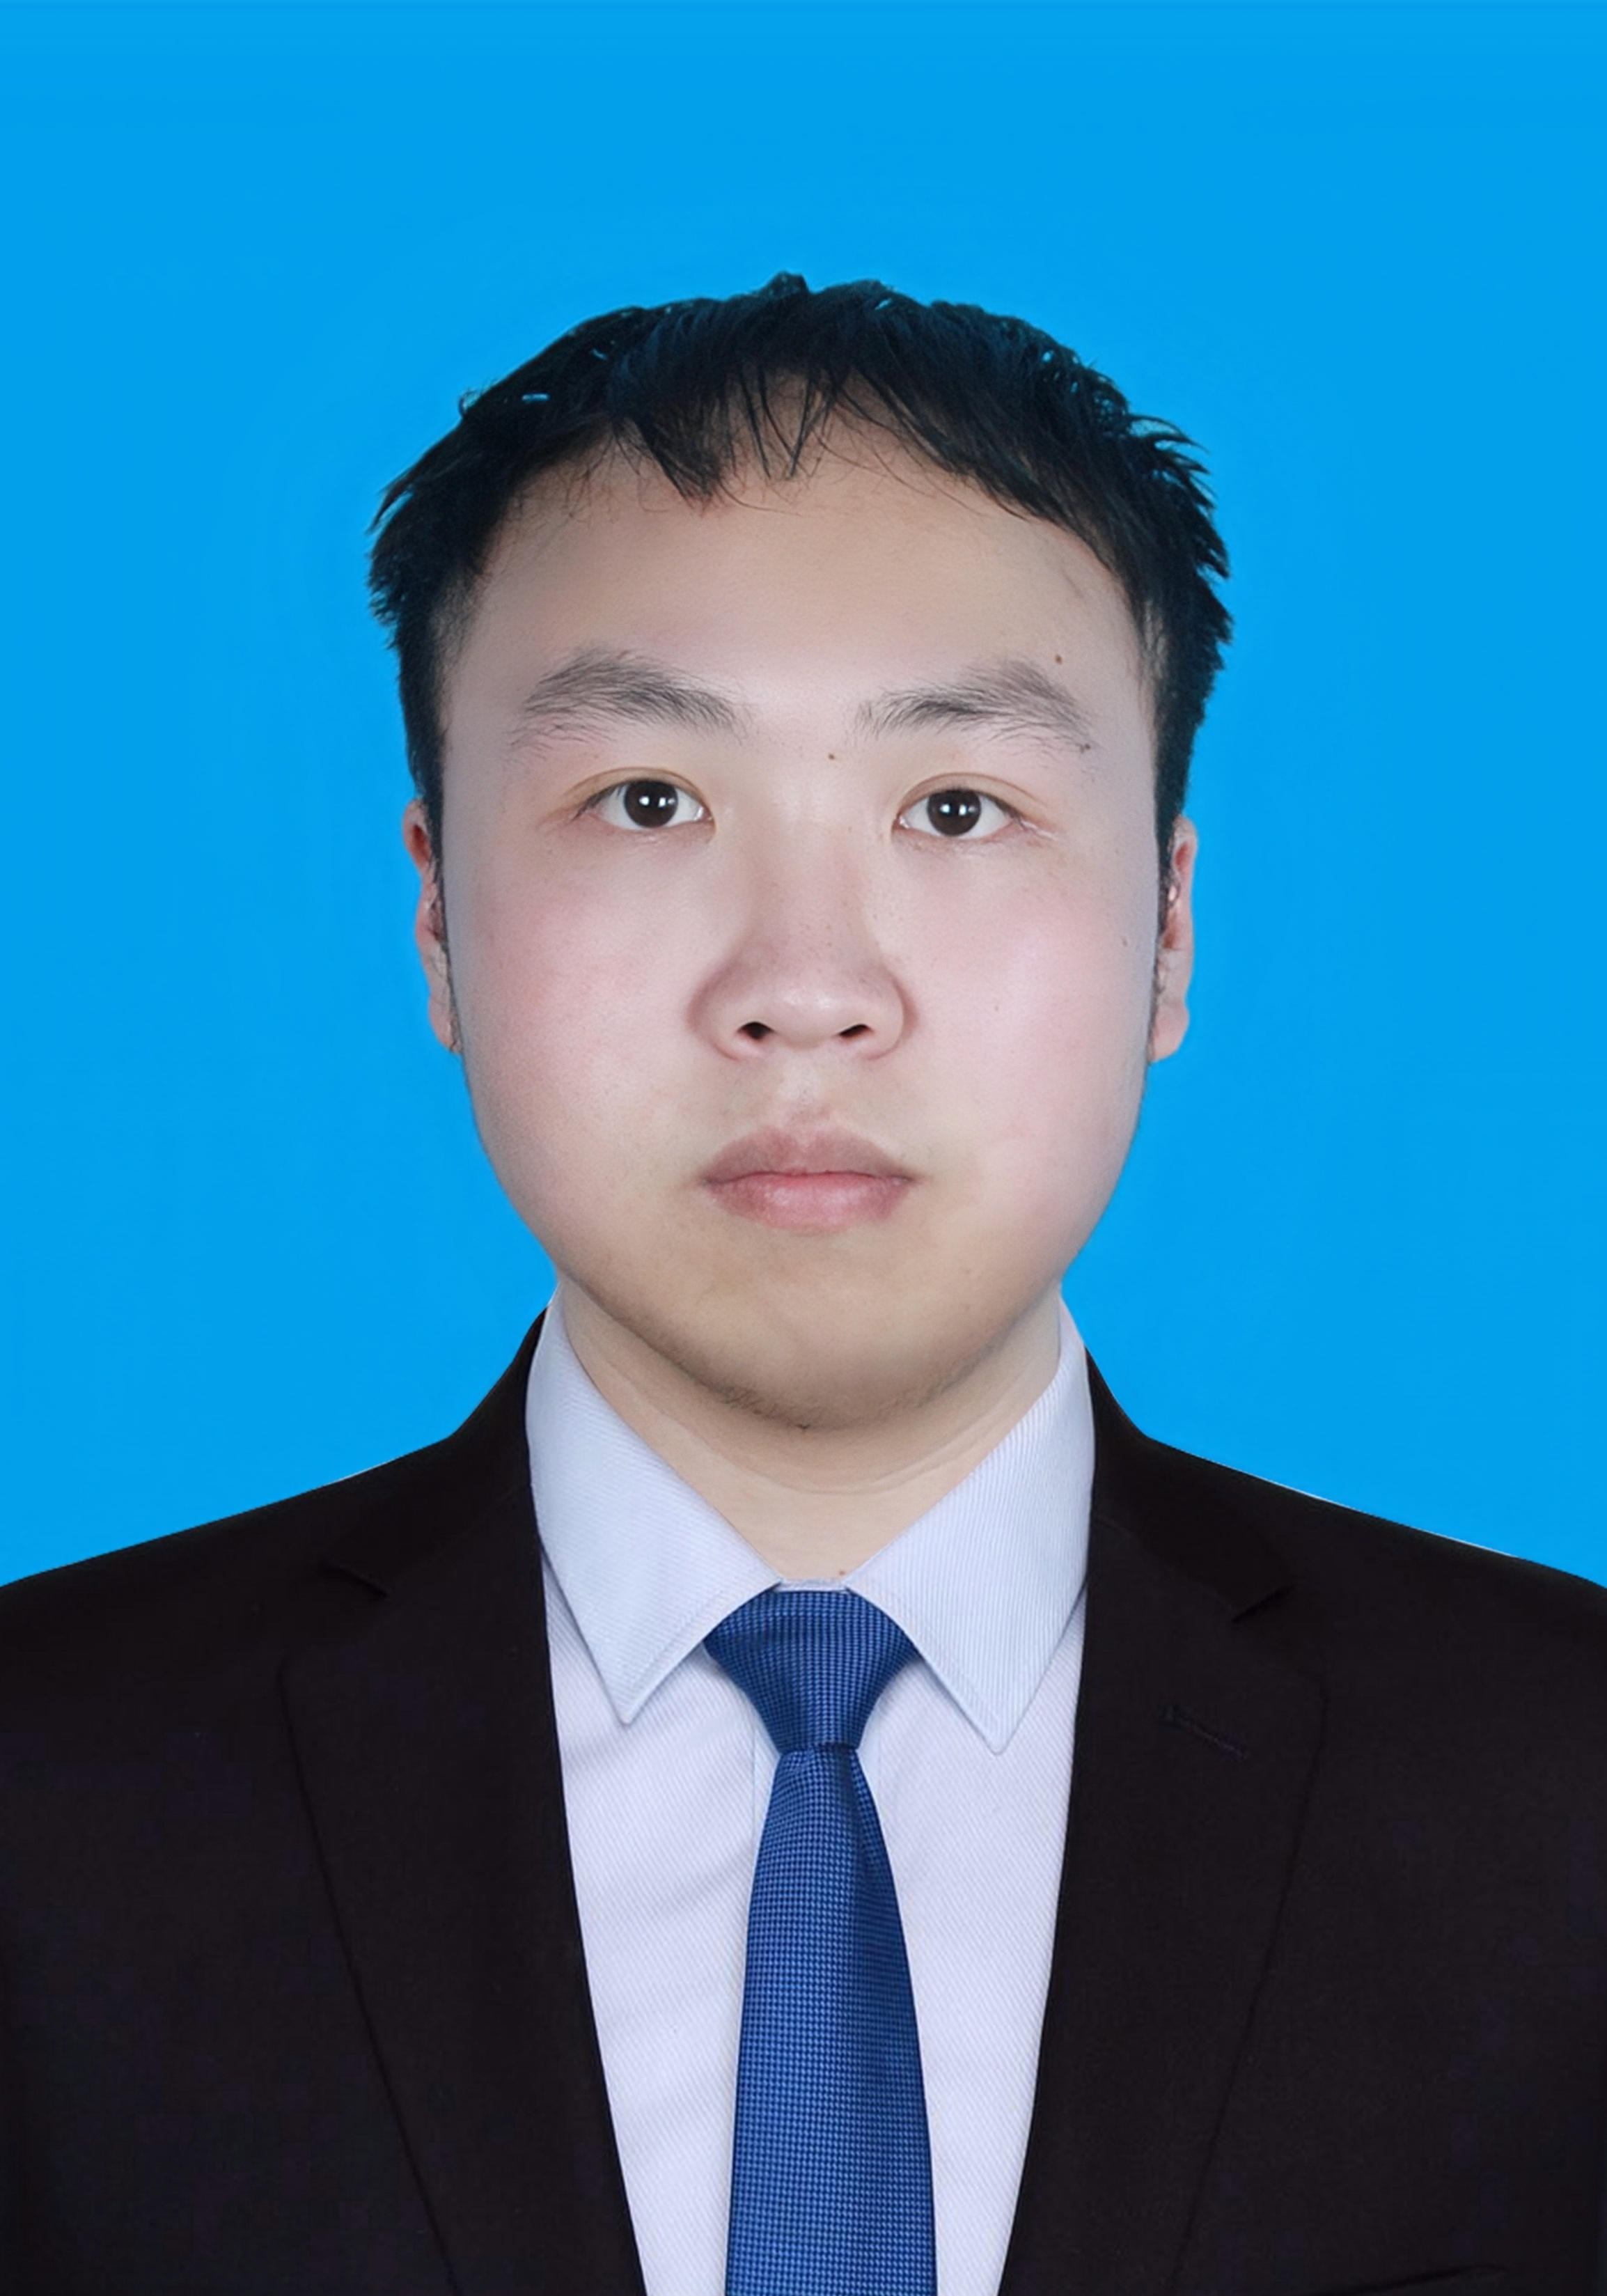
\includegraphics[width=0.4\linewidth]{../image.jpg}
  \end{minipage}
\end{center}

\section*{教育背景}
{
  \begin{itemize}[leftmargin=2em]
    \item 2023年9月--至今,衡阳师范学院,硕士,电子信息,导师:李浪教授,进行密码算法软硬件优化实现等研究。
    \item 2017年9月--2021年6月,长沙学院,本科,机械设计制造及其自动化。
  \end{itemize}

}

\section*{个人技能}
{
  \begin{itemize}[leftmargin=2em]
    \item \textbf{语言}: 常用 C, Python, \LaTeX; 熟悉 Verilog, Assembly, Rust;了解 C++, Java, TypeScript。
    \item \textbf{科研工具与环境}: Linux, Shell, Vim, VS Code, Git, GitHub等。
  \end{itemize}
}

\section*{科研成果}
\noindent 1) 论文
\begin{enumerate}[leftmargin=2em]
  \item \textbf{Jiahao Xiang}, Lang Li$^*$. Efficient implementations of CRAFT cipher for Internet of Things[J]. \textit{Computers and Electrical Engineering}, 2024, 116: 109168. (中科院3区, IF=4.0).
  \item \textbf{Jiahao Xiang}, Lang Li$^*$. Low-Latency Implementation of Bitsliced SPN-Cipher on IoT Processors. \textit{IEEE Transactions on Computers}. (CCF-A, 一审).
  \item \textbf{Jiahao Xiang}, Lang Li$^*$. Thread-Adaptive: Optimized Parallel Architectures of SLH-DSA on GPUs. (拟投 \textit{IEEE Transactions on Circuits and Systems II: Express Briefs}, 已完初稿).
  \item Lianrui Deng, Liang Li$^*$, Yu Ou, \textbf{Jiahao Xiang}. Tripm: a multi-label deep learning SCA model for multi-byte attacks[J]. \textit{International Journal of Machine Learning and Cybernetics}, 2025: 1-16.
  \item Xingqi Yue, Liang Li$^*$, Quiping Li, \textbf{Jiahao Xiang}, Zhiwen Hu. QLW: a lightweight block cipher with high diffusion[J]. \textit{The Journal of Supercomputing}, 2025, 81(1): 224.
\end{enumerate}

\noindent 2) 主持项目

\begin{enumerate}[leftmargin=2em]
  \item 湖南省研究生科研创新项目 ``轻量级分组密码的软硬件优化研究与实现'',编号:CX20240977。
\end{enumerate}

\end{document}
